\laborator{Основы математического пакета Mathcad}

\goal ознакомиться с пользовательским интерфейсом математического пакета Mathcad; изучить способы задания различного типа переменных и функций; освоить приемы работы с графическим и текстовым редакторами.

Mathcad --- программное средство, являющееся средой для выполнения на компьютере разнообразных математических расчетов. Mathcad включает множество операторов, встроенных функций и алгоритмов решения  математических задач. Пользовательский интерфейс системы создан так, что пользователь, имеющий элементарные навыки работы с Windows-приложениями, может сразу начать работу с Mathcad. Элементы управления расположены в меню в виде ленты, широко применяемой в офисных программных продуктах. Mathcad позволяет интегрировать математические расчеты и их графическое представление в рамках одного документа.

Лента меню содержит следующие пункты:
\begin{itemize}
	\item \menu[,]{Математика} --- содержит базовый функционал создания вычислительных блоков;
	\item \menu[,]{Ввод/вывод} --- позволяет осуществлять импорт исходных данных или экспорт результатов расчетов во внешние файлы;
	\item \menu[,]{Функции} --- содержит встроенные функции, сгруппированные по областям применения;
	\item \menu[,]{Матрицы/таблицы} --- позволяет создавать таблицы и матрицы и содержит функции обработки векторов и матриц;
	\item  \menu[,]{Графики} --- позволяет создавать графики и редактировать их внешний вид.
	\item \menu[,]{Формирование формул} --- позволяет из изменять внешний вид формул (шрифт, размер шрифта, числовой вид представления и т.д.);
	\item \menu[,]{Формирование текста} --- позволяет из изменять внешний вид текстовой области;
	\item \menu[,]{Расчет} --- позволяет изменять внутренние переменные точности и сходимости численных вычислений, отключать и включать вычисления в блоках;
	\item \menu[,]{Документ} --- позволяет изменять внешний вид документа (размеры отступов, межстрочного интервала, колонтитулы и т.д.);
	\item \menu[,]{Ресурсы} --- содержит справочный материал по встроенным функциям и учебные материалы.
\end{itemize} 

По умолчанию ввод осуществляется в вычислительный блок. Для запуска формульного редактора достаточно установить курсор мыши в любом свободном месте окна редактирования и щелкнуть левой клавишей. Появится визир в виде крестика. Его можно перемещать клавишами перемещения курсора. Визир указывает место, с которого можно начинать набор формул --- вычислительных блоков. Для ввода данных можно указать курсором мыши на нужный шаблон данных и щелчком левой ее клавиши ввести его.


\subsubsection*{Переменные}
Используемые в расчете данные хранятся в переменных. Чтобы определить переменную, необходимо выполнить следующие действия:
\begin{itemize}
	\item набрать имя переменной (регистр имеет значение);
	\item ввести оператор присваивания «:=», сделать через меню  \menu[,]{Математика, Операторы, Определение},  либо с помощью клавиши \keys{:};
	\item на место маркера, появившегося справа от оператора присваивания, ввести значение переменной;
	\item также можно ввести размерность переменной.
\end{itemize}
Mathcad позволяет работать со следующими типами переменных:
\begin{itemize}
\item скалярная величина;
\item вектор (который также может быть задан с помощью оператора ранжированной переменной);
\item матрица.
\end{itemize}

Работа в Mathcad осуществляется аналогично программированию на языках интерпретаторах, т.е. программа выполняется слева направо и сверху вниз. Это означает, что переменные должны быть определены в тексте программы левее или выше места их использования. Отделение десятичной части чисел, так же как и в большинстве языков программирования осуществляется через точку.
\begin{center}
	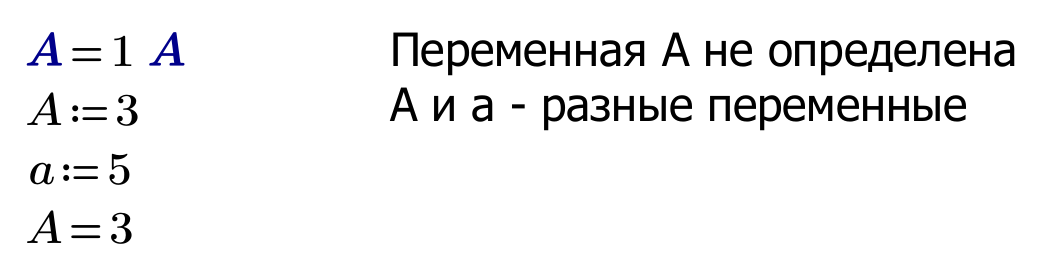
\includegraphics{new-var1.png}
\end{center}

При задании имен переменных рекомендуется исходить из обозначения данной величины в используемых формулах, и не использовать кириллических символов. При этом нельзя использовать одно и то же обозначение для различных переменных. В качестве примера можно привести следующее: для плотности газа $\rho_g$ и плотности жидкости $\rho_l$ можно использовать индексы. Греческие символы можно найти в меню  \menu[,]{Математика, Символы}. Индекс для скалярной величины можно задать в пункте меню \menu[,]{Математика, Стиль, Нижний индекс} при этом в данном случае индекс будет восприниматься программой как часть имени, и не следует путать его с индексом векторов и матриц.
\begin{center}
	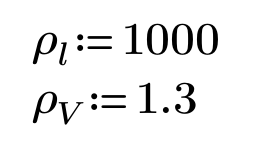
\includegraphics{new-var2.png}
\end{center}


\subsubsection*{Единицы измерения}
В пакете Mathcad имеется полный набор единиц измерения по международной системе СИ,  американской системе единиц  (USCS) и системе "сантиметр-грамм-секунда" (СГС). Использование единиц измерения для значений в расчете позволяет автоматически проводить определение размерности результирующей величины. Это позволяет значительно снизить ошибки, возникающие при переводе единиц измерения. Поэтому, при решении практических задач рекомендуется задавать размерности для всех используемых величин.

Для задания размерности необходимо при присвоении значения переменной дописать размерность данной величины. Список единиц измерения можно посмотреть в меню \menu[,]{Математика, ЕИ, ЕИ}

Mathcad автоматически проводит пересчет 
\begin{center}
	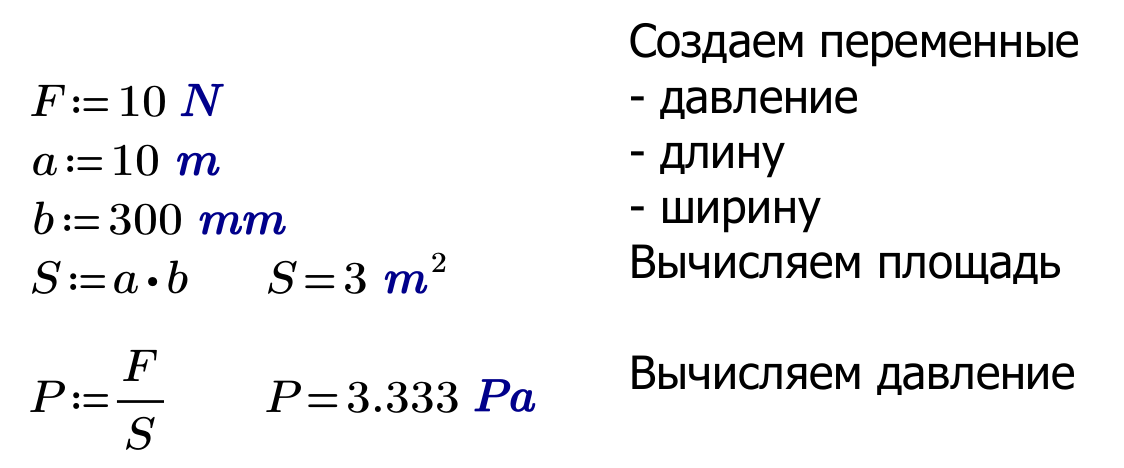
\includegraphics{new-ed-izm.png}
\end{center}

\subsubsection*{Матрицы и таблицы}
Массивы (векторы, матрицы), по принципу задания их элементов, можно разделить на две группы:
\begin{itemize}
\item векторы и матрицы, при задании которых не существует прямой связи между величиной элемента и его индексами;
\item ранжированные переменные --- векторы, величина элементов которых напрямую определяется индексом.
\end{itemize}
В Mathcad реализовано несколько способов задания массивов:
\begin{itemize}
	\item задание матрицы или вектора вручную с помощью команды \menu[,]{Матрицы/таблицы, Вставить матрицу};
	\item определение матрицы последовательным заданием каждого элемента;
	\item использование ранжированных переменных;
	\item создание таблицы данных;
	\item чтение из внешнего файла, и др.
\end{itemize}

Наиболее простым способом задания матрицы является использованием меню \menu[,]{Матрицы/таблицы, Вставить матрицу} или сочетанием клавиш \keys{\ctrl+M}. Изменять количество рядов и строк в матрице можно соответствующими командами в меню или сочетаниями клавиш: \keys{\shift+\enter} --- вставить столбец,   \keys{\shift+space} --- вставить строку.

Элементы матрицы могут быть как числами, так и выражениями. Если среди выражений или символов, выступающих в качестве элементов матрицы, есть неизвестные или параметры, то они обязательно должны быть численно определены выше.


В случае заданной матрицы всегда можно получить значение любого его элемента, используя его матричные индексы. Матричные индексы равняются номеру строки и столбца, на пересечении которых элемент находится. В математике отсчет строк и столбцов принято начинать с единицы. В программировании же начальные индексы обычно равняются нулю. По умолчанию в Mathcad нумерация строки и столбцы тоже начинаются с нуля. В том случае если такая система не удобна, то точку отсчета можно изменить через переменную \mc{ORIGIN} на панели  \menu[,]{Расчет} или переопределив переменную в самом документе.

Чтобы получить значение какого-то матричного элемента, нужно ввести имя матрицы с соответствующими индексами. Для задания индексов  в меню \menu[,]{Матрицы/таблицы, Операторы с матрицами, Индекс матрицы}, которой соответствует клавиша \keys{[}. Нажав ее, вы увидите, что на месте будущего индекса, чуть ниже текста имени матрицы, появится маркер ввода индекса. В него через запятую следует ввести значения индексов. На первом месте при этом должен стоять номер строки, а на втором --- номер столбца. При выделении элемента вектора нужно задать только индекс строки. Индексы также могут быть определены и через выражения или специальные функции.
\begin{center}
	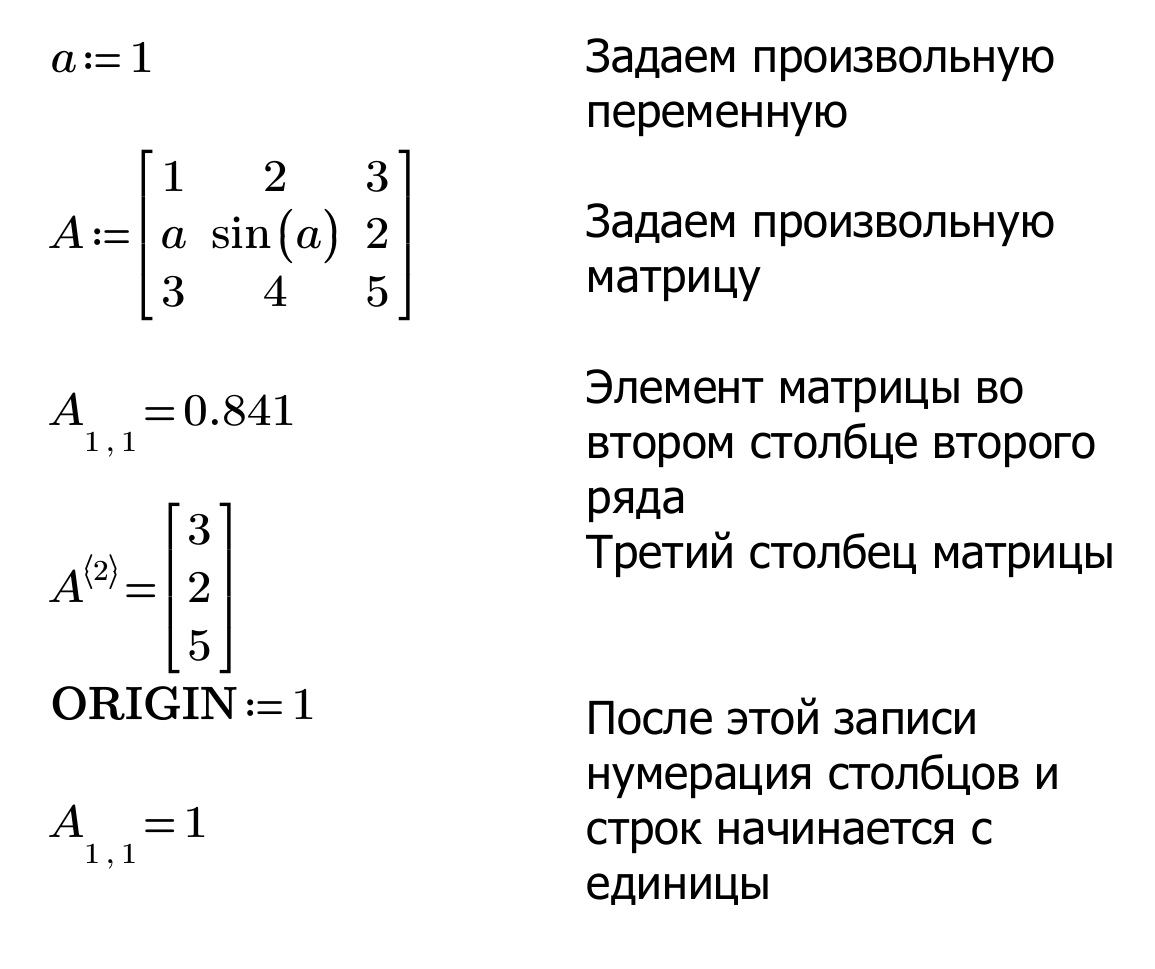
\includegraphics{new-mat1.png}
\end{center}


Помимо одного элемента можно очень просто выделить и целые матричные столбцы или строки. Чтобы это сделать, нужно использовать специальные операторы в меню \menu[,]{Операторы с матрицами} (также вводится сочетанием \keys{\ctrl+\shift+C} и \keys{\ctrl+\shift+R}  соответственно)  и в маркер ввести требуемый номер столбца или строки.

При вычислении значений по одной и той же формуле, необходимо использовать оператор векторизации расположенный в меню \menu[,]{Матрицы/таблицы, Операторы с матрицами} или по горячим клавишам \keys{\ctrl+\shift+\textasciicircum}. При этом вычисление выражения, записанного под знаком векторизации, будет проводится поэлементно. Без оператора векторизации соответственно будут проводиться матричные операции.
\begin{center}
	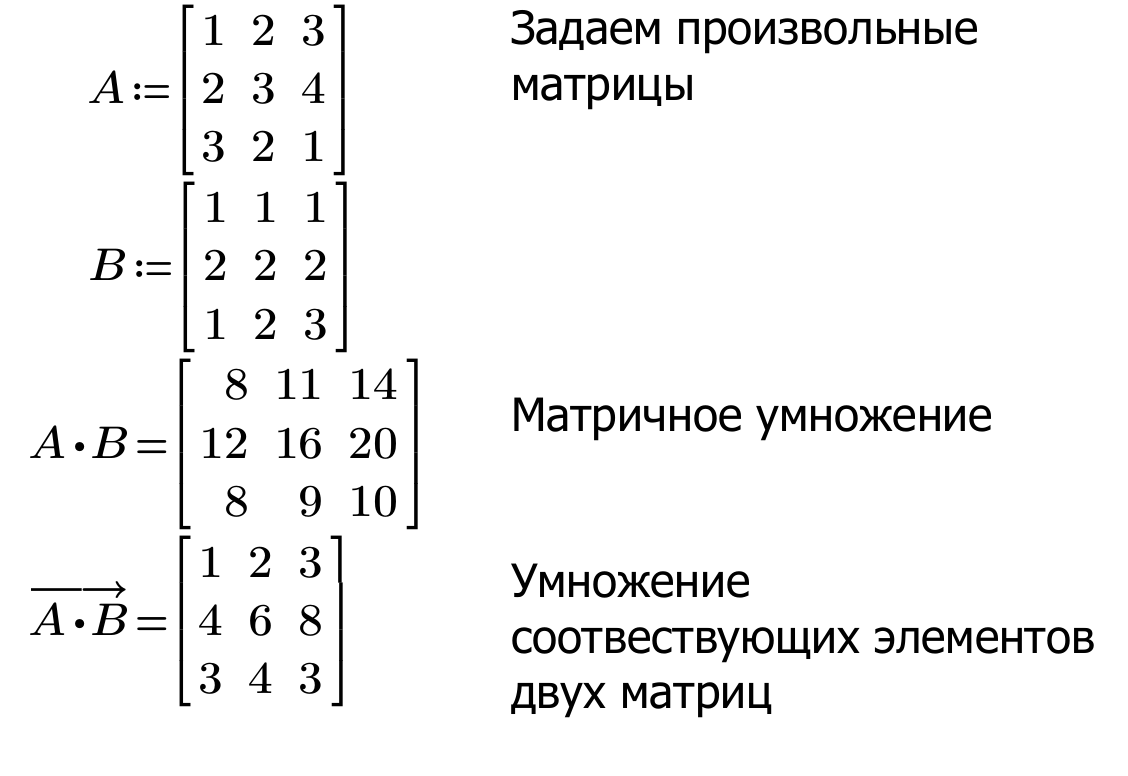
\includegraphics{new-mat2.png}
\end{center}


%пример

Одной из разновидностей задания массивов является использование так называемых ранжированных переменных. Ранжированная переменная --- это разновидность вектора, особенностью которого является непосредственная связь между индексом элемента и его величиной. В Mathcad ранжированные переменные очень активно используются как аналог программных операторов цикла (например, при построении графиков).

Простейшим примером ранжированной переменной является вектор, значение элементов которого совпадает с их индексами. Для задания такой ранжированной переменной выполните следующую последовательность действий:
\begin{itemize}
	\item Введите имя переменной и оператор присваивания.
	\item  Выберите  \menu[,]{Математика, Операторы, Область дискретных значений}. При этом будет введена заготовка в виде двух маркеров, разделенных точками.	Данную заготовку можно вставить дважды нажав на клавишу \keys{.}.
	\item В левый  маркер заготовки ранжированной переменной введите ее первое значение, в правый – последнее.
\end{itemize}

Шаг изменения ранжированной переменной при ее задании с помощью описанного способа постоянен и равен единице. Однако при необходимости его можно сделать и произвольным. Дли этого нужно, поставив после левой границы интервала запятую, ввести второе значение ранжированной переменной. Разность между первым и вторым ее значением и определит шаг. 
\begin{center}
	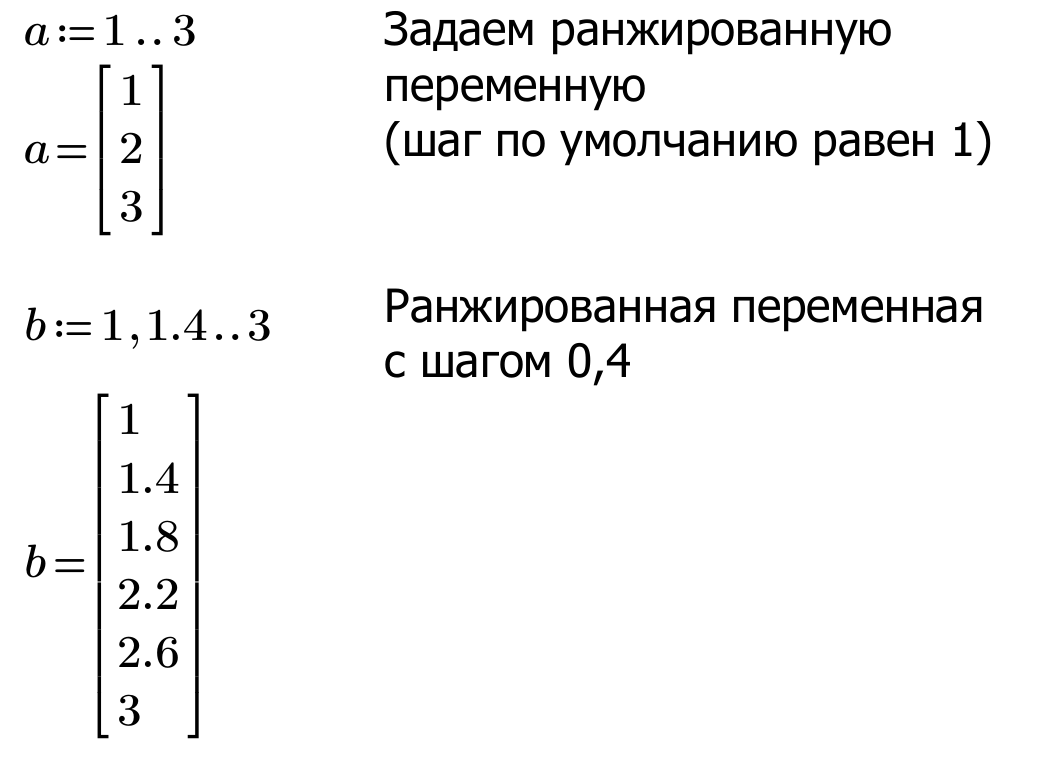
\includegraphics{new-mat3.png}
\end{center}

Использование ранжированных переменных во многом основано на том, что большинство математических действий в Mathcad над векторами осуществляется точно так же, как над простыми числами. Так, например, существует возможность вычисления значений практически любой встроенной и пользовательской функции от вектора. 

\subsubsection*{Таблицы}
Часто экспериментальные данные обрабатываются в Mathcad в виде матриц. Однако использовать описанные выше стандартные методы задания массивов для этого крайне неудобно. В этом случае можно использовать таблицу ввода. Для этого необходимо выбрать пункт \menu[,]{Матрицы/Таблицы, Вставить таблицу} или начать сочетание клавиш \keys{\ctrl + 6}. Добавление или удаление строк таблицы осуществляется так же как и для матриц. Каждому столбцу таблицы можно присвоить имя переменной и размерность величины.
\begin{center}
	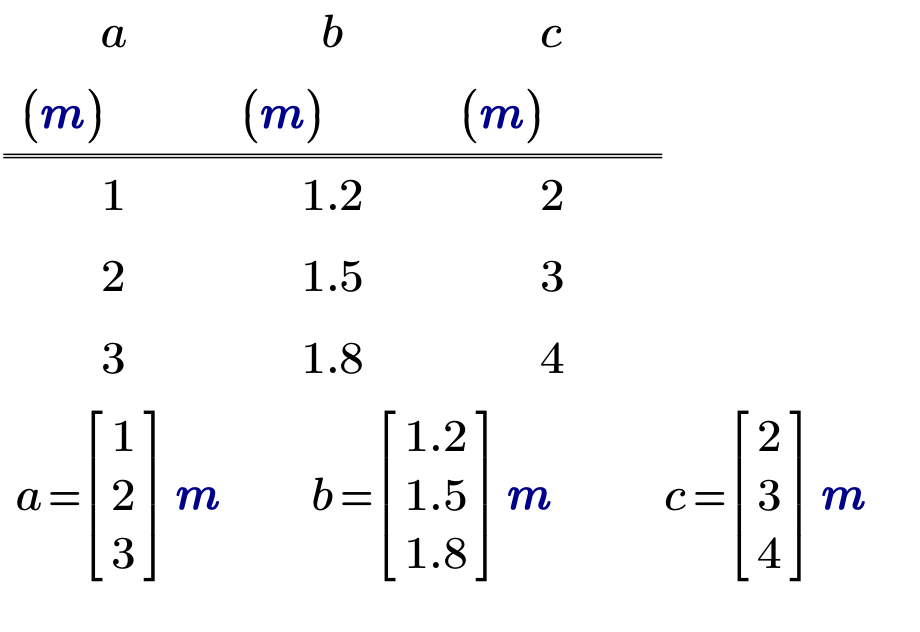
\includegraphics{new-tab1.png}
\end{center}


\subsubsection*{Функции}
Функции в Mathcad делятся на две группы:
\begin{itemize}
\item функции пользователя;
\item встроенные функции.
\end{itemize}
Техника использования функций обоих типов абсолютно идентична, а вот задание отличается принципиально. Для задания функции пользователя необходимо выполнить следующие действия:
\begin{itemize}
	\item ввести имя функции;
	\item после имени ввести пару круглых скобок, в которых через запятую необходимо указать все переменные, от которых зависит функция;
	\item ввести оператор присваивания \mc{:=};
	\item на место черного маркера, появившегося справа от оператора присваивания, необходимо задать вид функции.
\end{itemize}

В выражение определяемой функции могут входить как непосредственно переменные, так и другие встроенные и пользовательские функции. 

Встроенные функции --- это функции, заданные в Mathcad изначально. Чтобы их использовать, достаточно корректно набрать имена функций с клавиатуры. Наиболее распространенные функции представлены в меню \menu[,]{Функции}. Также в этом меню можно вызвать список всех встроенных функций в пункте  \menu[,]{Функции, Все функции}.
\begin{center}
	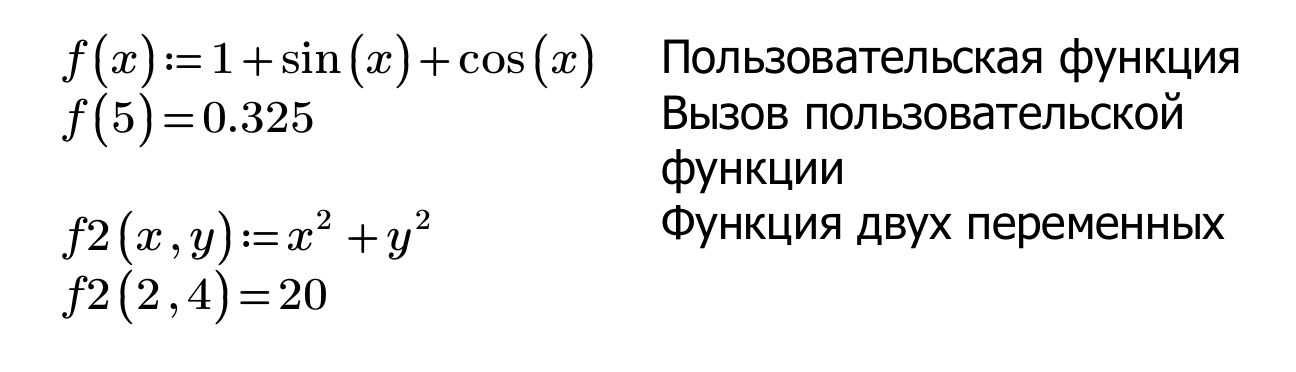
\includegraphics{new-fun1.png}
\end{center}


\subsubsection*{Текстовый редактор}

Текстовый режим в Mathcad позволяет создавать всевозможные комментарии и качественно оформлять решенные задачи.
Чтобы ввести текстовую область, выберите пункт \menu[,]{Математика, Текстовое поле} или  нажмите сочетание клавиш \keys{\ctrl + T} (курсор ввода при этом должен располагаться на чистом участке документа). При этом появится специальная рамка.
Набирается текст в Mathcad точно так же, как в любом текстовом редакторе. Если известно, сколько места на листе займет комментарий, то можно сразу растянуть текстовую область до нужных размеров. Можно выбрать пункт  \menu[,]{Математика, Блок текста} (или сочетание клавиш  \keys{\ctrl+ \shift + T}) и область ввода текста займет всю ширину страницы.

\subsubsection*{Графический редактор}
Все основные типы графиков и инструменты работы с ними расположены на панели \menu[,]{Графики}. Для построения графика необходимо нажать на кнопку  \menu[,]{Вставить график} и из выпадающего  меню выбрать тип графика, в документе появится область с координатными осями. В осях необходимо указать векторы, содержащие данные по которым строится график. 
Добавить или удалить график с координатной оси можно соответствующими кнопкам на панели \menu[,]{Графики} (или сочетанием клавиш \keys{ \shift + \enter} и \keys{\del} )

На панели расположено меню, позволяющее изменять внешний вида графика (типа, толщины и цвета линии; добавления и изменения вида маркеров, фон и т.д.). 
\begin{center}
	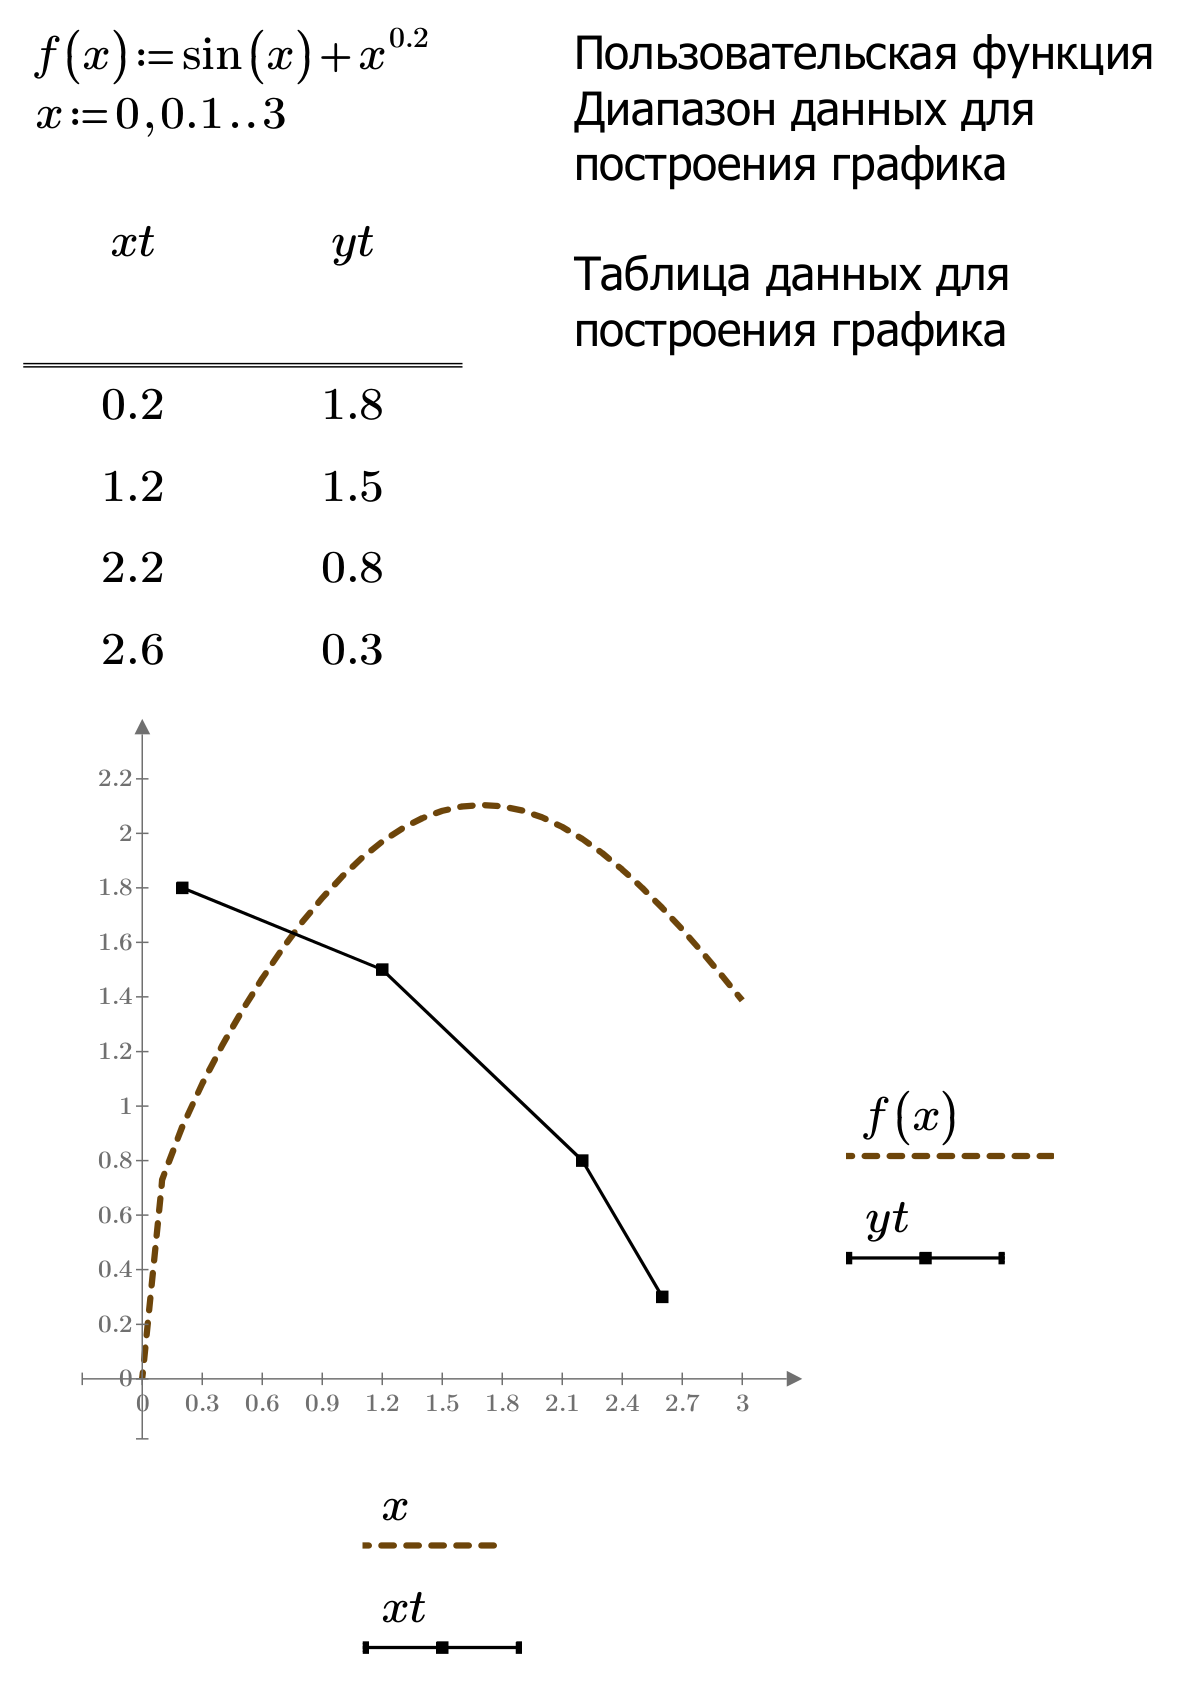
\includegraphics{new-plot1.png}
\end{center}


\subsubsection*{Символьные вычисления}
В Mathcad имеются возможности символьных вычислений: решение уравнений, преобразования, разложения и т.д. Для аналитического преобразования можно воспользоваться кнопкой $\rightarrow$ на панели  \menu[,]{Графики, Математика, Символьные вычисления} или сочетанием \keys{\ctrl + .}. С помощью аналитического преобразования возможно вычислить интегралы и производные функций.

Для аналитического решения уравнений необходимо нажать кнопку solve  на панели  \menu[,]{Графики, Математика, Символьные вычисления}. В документе появится стрелка с надписью solve, левее стрелки необходимо ввести уравнение.


\begin{center}
	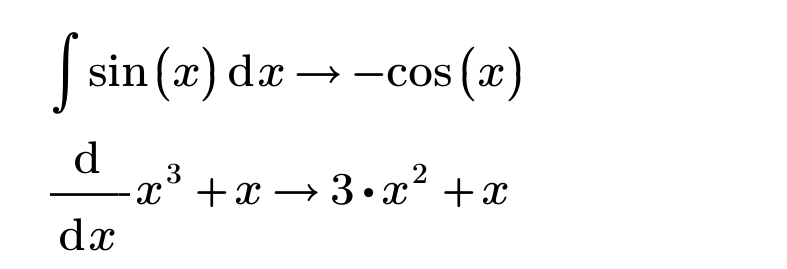
\includegraphics{new-symbol1.png}
\end{center}

\subsubsection*{Численное решение уравнений и систем уравнений}
Для численного поиска решений уравнений с одним неизвестным в Mathcad существует специальная встроенная функция \mc{root}. Эта функция может использоваться в двух различных формах, при этом реализуются разные численные алгоритмы. Так, если определена только одна точка приближения к корню, поиск решений будет осуществляться методом секущих. Если же задан интервал, на котором предположительно локализовано решение, то поиск его будет осуществлен с применением двух модификаций метода бисекции.

Если необходимо найти корень некоторого уравнения, причем известен интервал, в котором он локализован, проще всего использовать функцию \mc{root} с четырьмя аргументами: \mc{rоot(f(x), x, a, b)}, где \mc{f(x)} --- функция, определяющая уравнение, \mc{х} --- переменная, \mc{а} и \mc{b} --- границы интервала локализации. Обязательным условием является то, что значения функции на концах интервала должны быть противоположных знаков. Это связано с особенностью используемых \mc{root} алгоритмов. Если нарушить это условие, система выдаст сообщение об ошибке.

В тех случаях, когда определить границы такой локализации невозможно, следует применять функцию \mc{root} с одной точкой приближения: \mc{rоot(f(x), x)}. В этом случае необходимо перед вызовом функцию \mc{root} задать для переменной \mc{x} начальное приближение.

Важной характеристикой решения является его точность. В Mathcad можно регулировать величину погрешности решения, изменяя значение специальной системной переменной \mc{TOL} (на панели \menu[,]{Расчет}). В общем случае, чем меньше \mc{TOL}, тем точнее будет найдено решение, но и тем больше времени уйдет на его определение (а также будет выше риск, что численный метод не сойдется к решению).

%пример решения
\begin{center}
	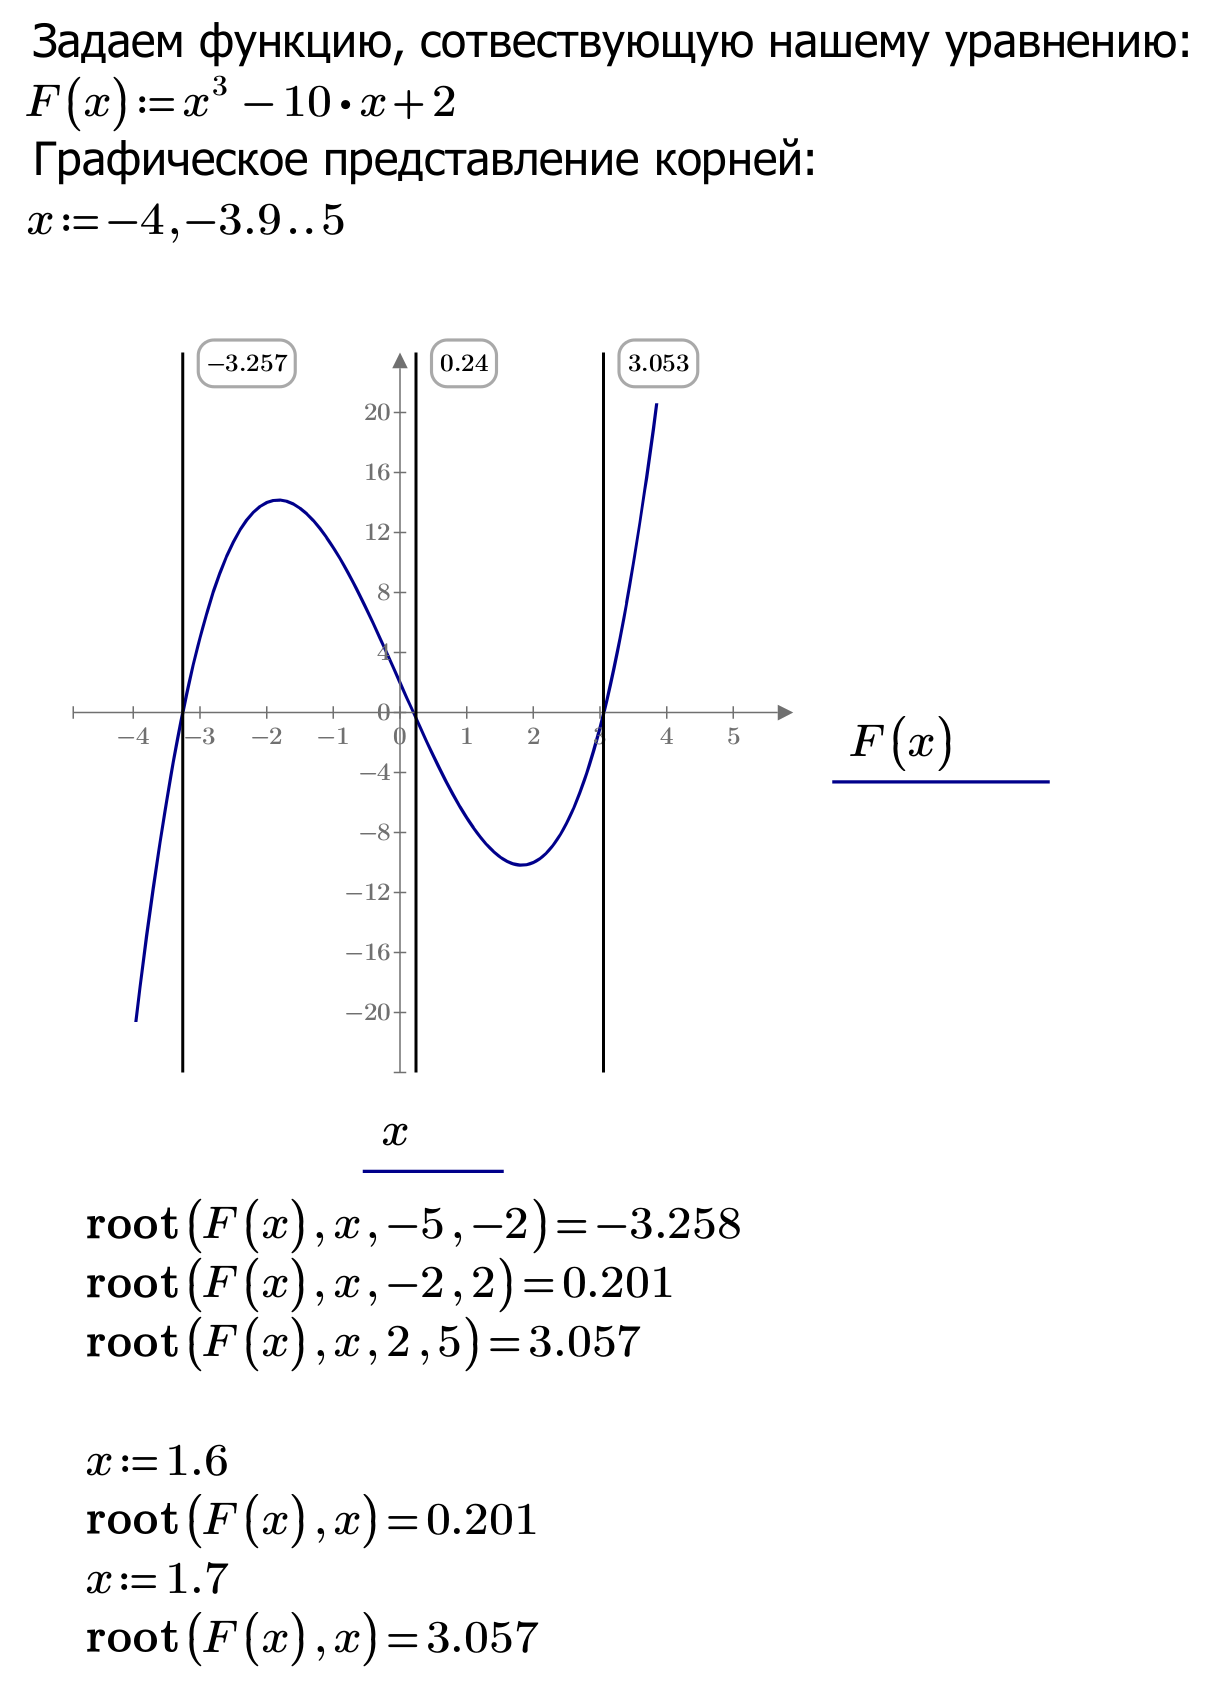
\includegraphics{new-eq1.png}
\end{center}

Для численного решения систем уравнений в Mathcad служит блок решения вызвать который можно с панели \menu [,] {Математика} или сочетанием клавиш \keys{\ctrl+1}. Используя блок решения, можно решать системы, содержащие до 250 нелинейных уравнений и до 1000 линейных. Результатом решения системы будет численное значение искомых корней.

Для решения системы уравнений с помощью блока решения необходимо:
\begin{itemize}
	\item Задать начальные приближения для всех неизвестных, входящих в систему уравнений. Mathcad решает уравнения при помощи итерационных методов. На основе начального приближения строится последовательность, сходящаяся к искомому решению.
	\item В области \mc{Ограничения} необходимо ввести уравнения и неравенства искомой системы. Для записи уравнений необходимо использовать знак \mc{Сравнение}, вызвать который можно с панели \menu [,] {Математика, Операторы} либо с помощью сочетания клавиш \keys{\ctrl+=}.
	\item В области \mc{Решатель} необходимо ввести функцию \mc{find}. В аргументах функции необходимо задать переменные в том порядке, в котором должны быть расположены в ответе соответствующие им корни. Если результаты решения требуется использовать в дальнейших расчетах, то тогда их необходимо присвоить некоторой переменной .
\end{itemize}

%пример решения
\begin{center}
	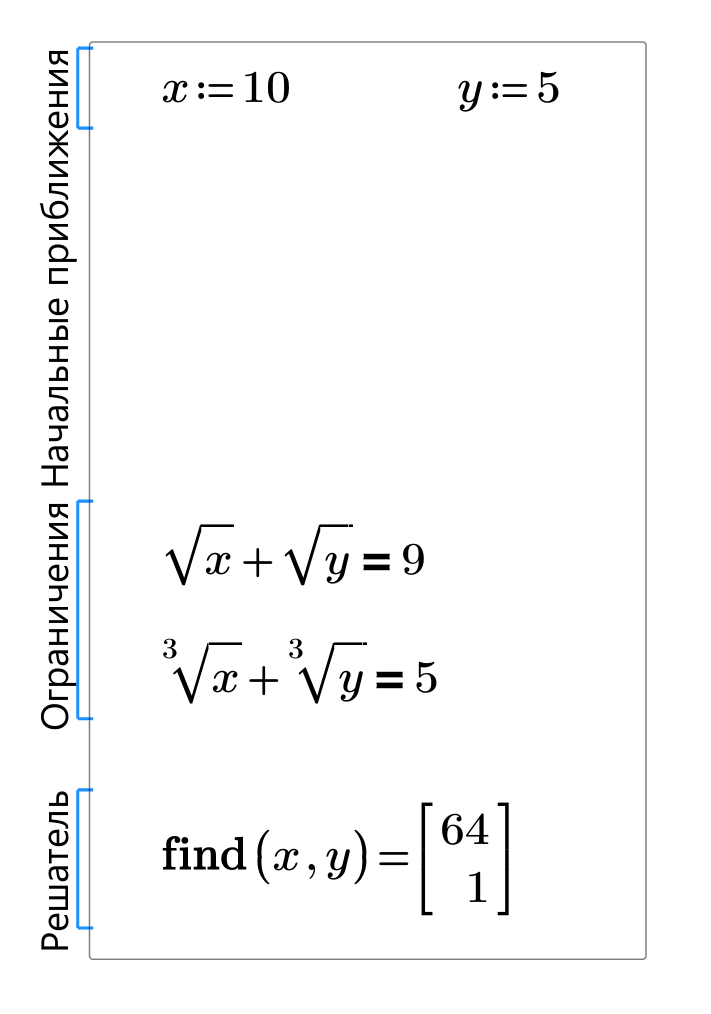
\includegraphics{new-eq2.png}
\end{center}


\subsubsection*{Вопросы для самоконтроля}
\begin{enumerate}
	\item Для каких целей предназначен математический пакет Mathcad?
	\item С какими типами переменных позволяет работать Mathcad?
	\item В чем разница между оператором присваивания и оператором численного решения?
	\item Какие типы функций есть в Mathcad, в чем их отличие?
	\item Для чего предназначен графический редактор?
	\item Для чего предназначен текстовый редактор?
	\item Что является результатом решения системы нелинейных уравнений?
	\item Какие символы должны использоваться в качестве знаков равенства или неравенства при записи уравнений в блоке решения?
\end{enumerate}



